\pdfminorversion=4
\documentclass[aspectratio=169]{beamer}

\mode<presentation>
{
  \usetheme{default}
  \usecolortheme{default}
  \usefonttheme{default}
  \setbeamertemplate{navigation symbols}{}
  \setbeamertemplate{caption}[numbered]
  \setbeamertemplate{footline}[frame number]  % or "page number"
  \setbeamercolor{frametitle}{fg=white}
  \setbeamercolor{footline}{fg=black}
}

\usepackage[english]{babel}
\usepackage[utf8x]{inputenc}
\usepackage{tikz}
\usepackage{courier}
\usepackage{array}
\usepackage{bold-extra}
\usepackage{minted}
\usepackage[thicklines]{cancel}
\usepackage{fancyvrb}

\xdefinecolor{dianablue}{rgb}{0.18,0.24,0.31}
\xdefinecolor{darkblue}{rgb}{0.1,0.1,0.7}
\xdefinecolor{darkgreen}{rgb}{0,0.5,0}
\xdefinecolor{darkgrey}{rgb}{0.35,0.35,0.35}
\xdefinecolor{darkorange}{rgb}{0.8,0.5,0}
\xdefinecolor{darkred}{rgb}{0.7,0,0}
\definecolor{darkgreen}{rgb}{0,0.6,0}
\definecolor{mauve}{rgb}{0.58,0,0.82}

\title[2019-09-14-awkward-strangeloop]{Jagged, ragged, awkward arrays}
\author{Jim Pivarski}
\institute{Princeton University -- IRIS-HEP}
\date{September 14, 2019}

\usetikzlibrary{shapes.callouts}

\begin{document}

\logo{\pgfputat{\pgfxy(0.11, 7.4)}{\pgfbox[right,base]{\tikz{\filldraw[fill=dianablue, draw=none] (0 cm, 0 cm) rectangle (50 cm, 1 cm);}\mbox{\hspace{-8 cm}
\includegraphics[height=1 cm]{princeton-logo-long.png}\hspace{0.1 cm}\raisebox{0.1 cm}{
\includegraphics[height=0.8 cm]{iris-hep-logo-long.png}}\hspace{0.1 cm}}}}}

\begin{frame}
  \titlepage
\end{frame}

\logo{\pgfputat{\pgfxy(0.11, 7.4)}{\pgfbox[right,base]{\tikz{\filldraw[fill=dianablue, draw=none] (0 cm, 0 cm) rectangle (50 cm, 1 cm);}\mbox{\hspace{-8 cm}
\includegraphics[height=1 cm]{princeton-logo.png}\hspace{0.1 cm}\raisebox{0.1 cm}{
\includegraphics[height=0.8 cm]{iris-hep-logo.png}}\hspace{0.1 cm}}}}}

% Uncomment these lines for an automatically generated outline.
%\begin{frame}{Outline}
%  \tableofcontents
%\end{frame}

% START START START START START START START START START START START START START

\begin{frame}{Motivation: particle physics analysis}
\Large
\vspace{0.23 cm}
\begin{columns}
\column{0.5\linewidth}
\only<1>{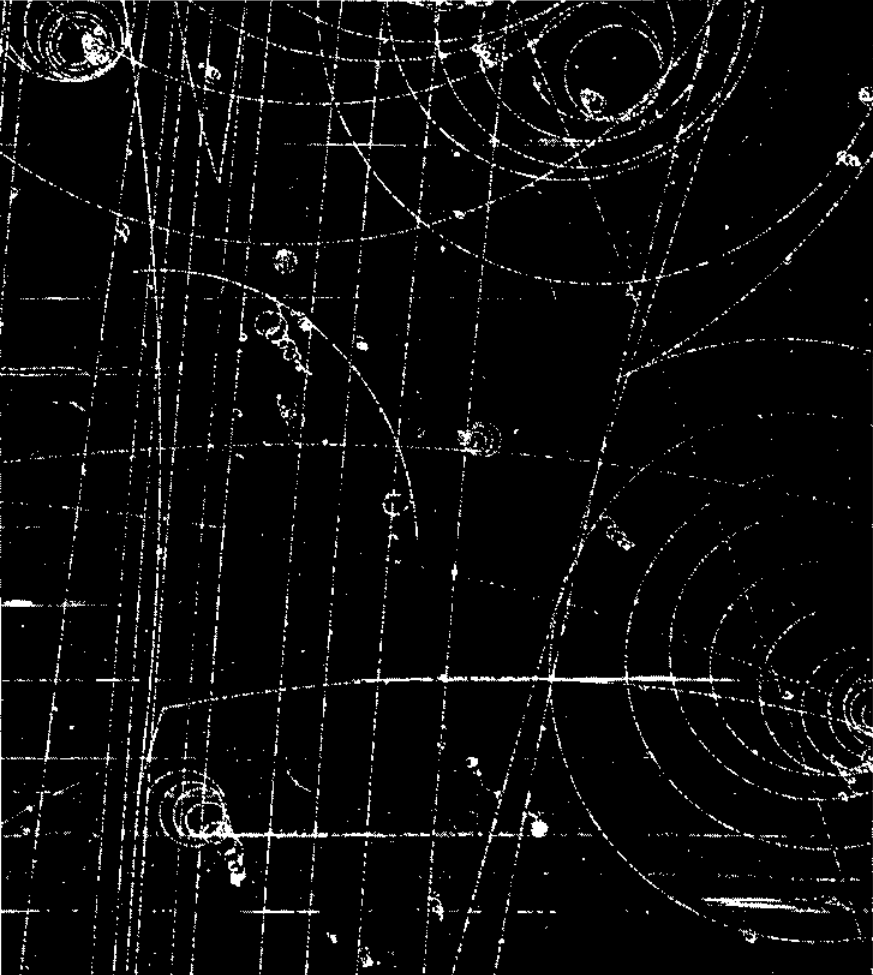
\includegraphics[width=\linewidth]{omega-minus-1.png}}\only<2->{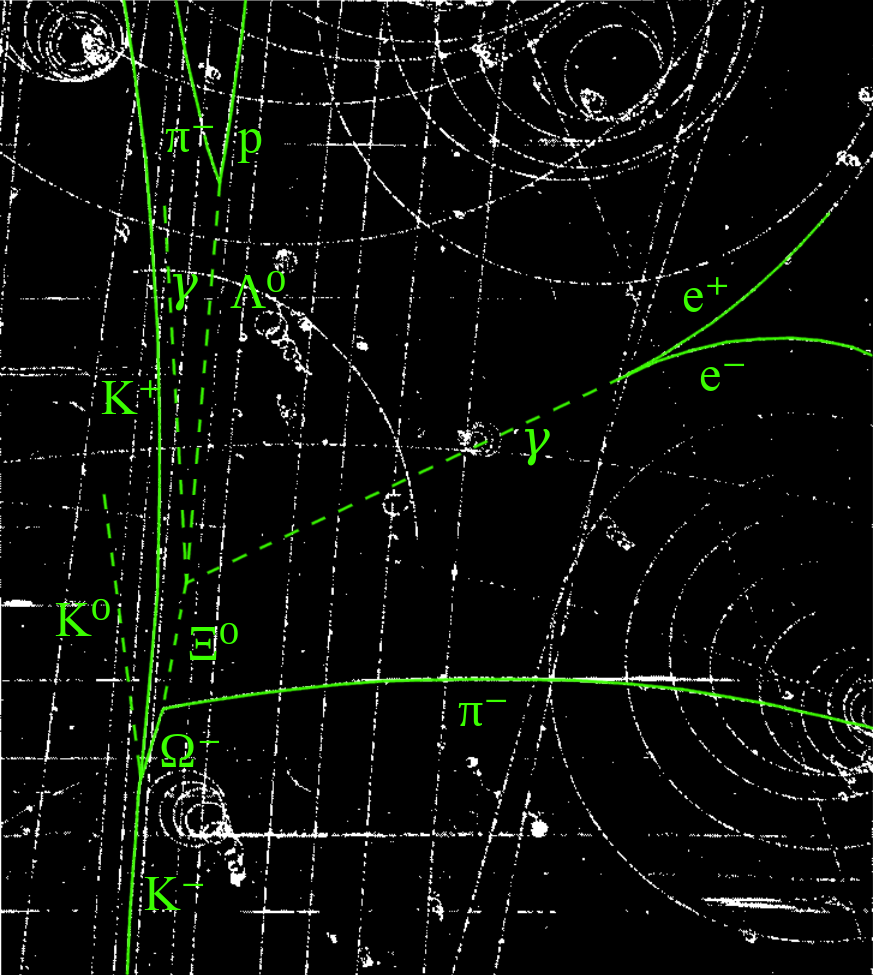
\includegraphics[width=\linewidth]{omega-minus-2.png}}
\column{0.5\linewidth}

\begin{center}
\begin{onlyenv}<1>
This is a famous photo: the 1964 discovery of the $\Omega$ baryon.

\vspace{1 cm}
Do you see it?

\vspace{1 cm}
\end{onlyenv}\begin{onlyenv}<2>
How about now?

\vspace{0.5 cm}
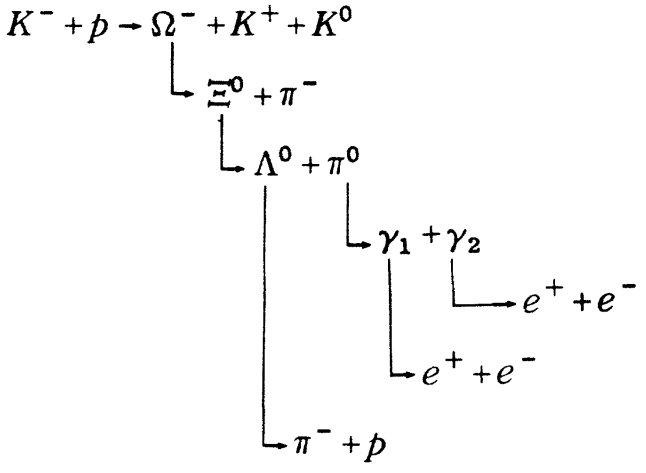
\includegraphics[width=\linewidth]{decay-chain.png}
%% \begin{align*}
%% K^- + p & \to \Omega^- + K^+ + K^0 \\
%% \Omega^- & \to \Xi^0 + \pi^- \\
%% \Xi^0 & \to \Lambda^0 + \pi^0 \\
%% \Lambda^0 & \to p + \pi^- \\
%% \pi^0 & \to \gamma + \gamma
%% \end{align*}

\vspace{1 cm}
\end{onlyenv}\begin{onlyenv}<3>
This is what particle physicists do: we collide particles, produce new ones and take pictures of their decay chains.

\vspace{1 cm}
However, these pictures come to us unlabeled: lots of interactions overlap the ``interesting'' ones.

\vspace{1 cm}
\end{onlyenv}
\end{center}

\end{columns}
\end{frame}

\begin{frame}{}
\begin{columns}
\column{1.15\linewidth}
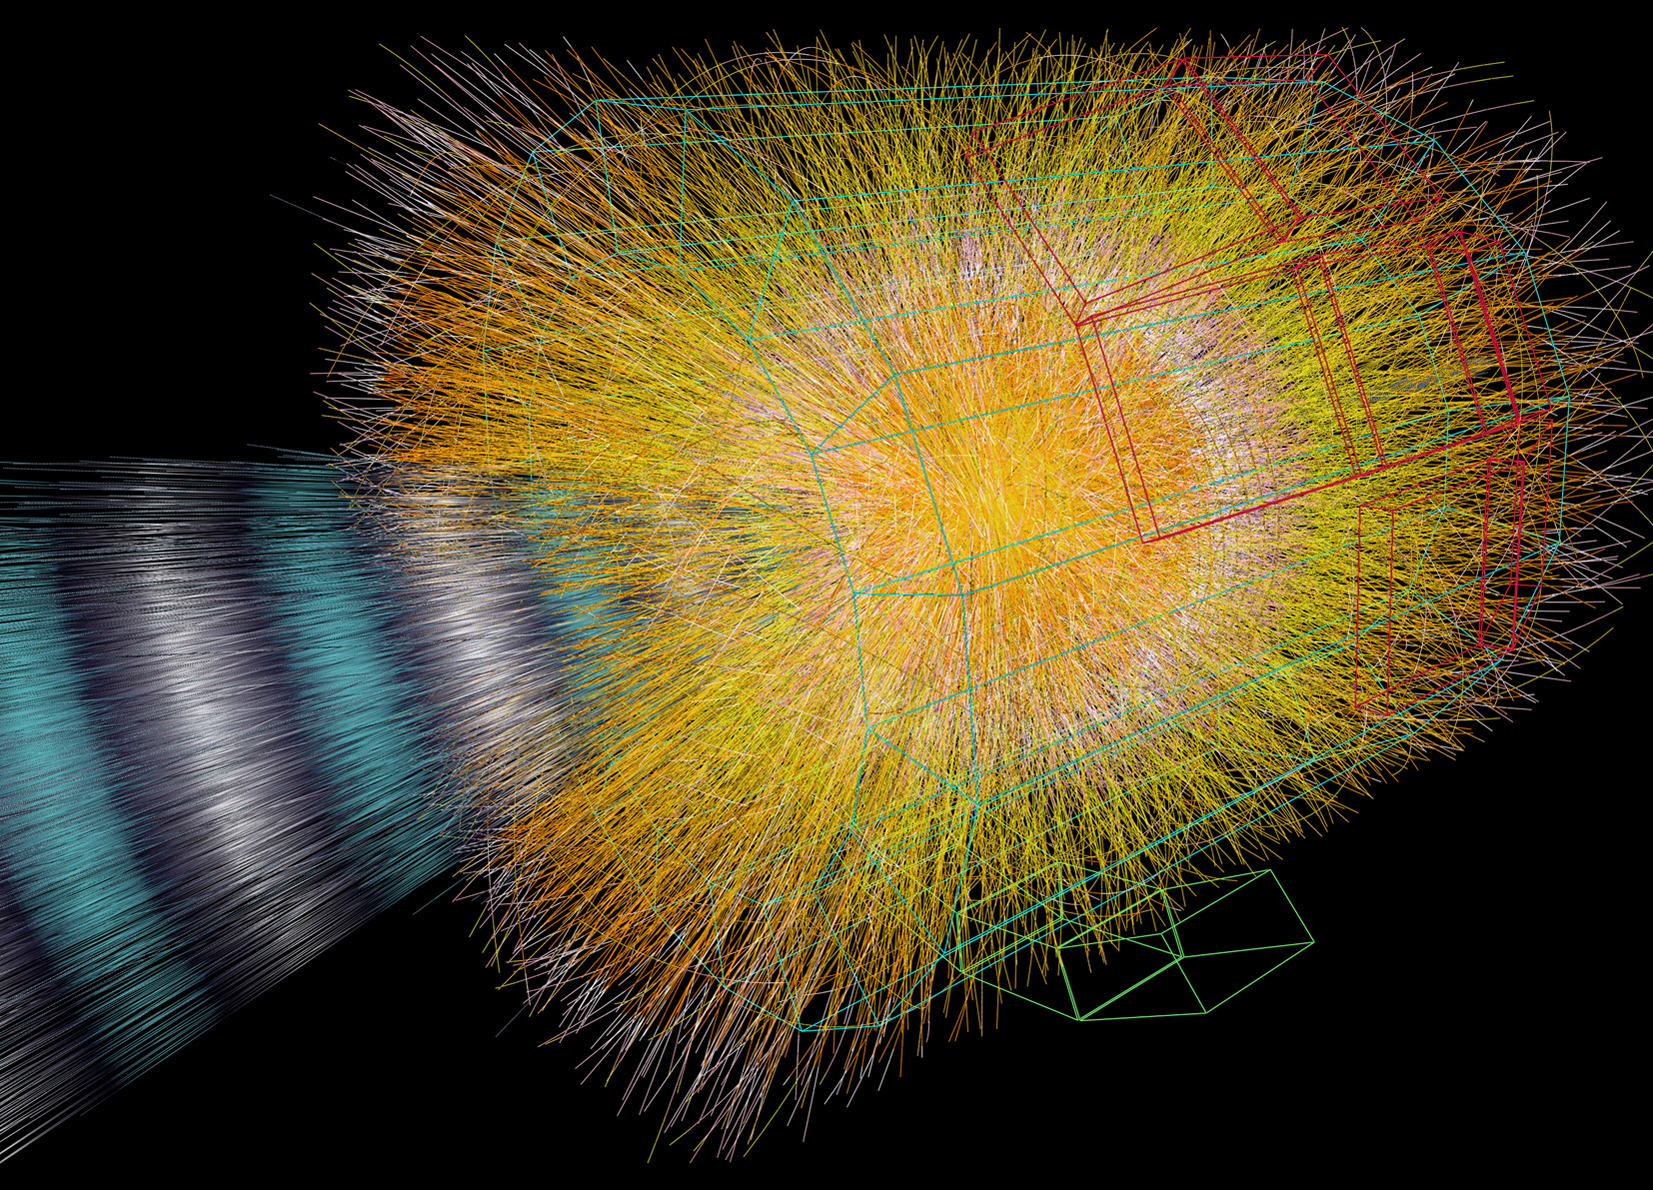
\includegraphics[width=\linewidth]{090324_ALICE-hirez.jpg}
\end{columns}
\end{frame}

\begin{frame}{Then and now: mostly just scale-up}
\vspace{0.15 cm}
\begin{columns}
\column{0.32\linewidth}
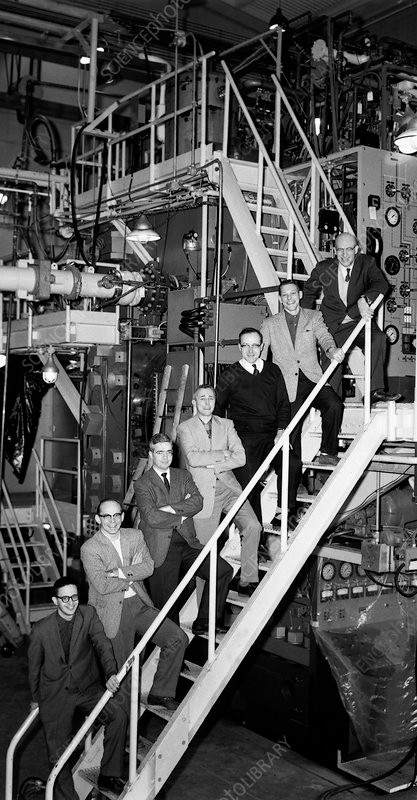
\includegraphics[width=\linewidth]{H4000010-Team_that_discovered_Omega_minus_particle.jpg}

\column{0.5\linewidth}
\begin{center}
\begin{columns}
\column{0.35\linewidth}
\centering
photographs

\vspace{0.5 cm}
100,000 events

\vspace{0.5 cm}
manual/semi-automated scans

\column{0.35\linewidth}
\centering
digitized signals \\

\vspace{0.5 cm}
$\sim$trillion events \\

\vspace{0.5 cm}
algorithmic searches and machine learning
\end{columns}
\end{center}

\column{0.32\linewidth}
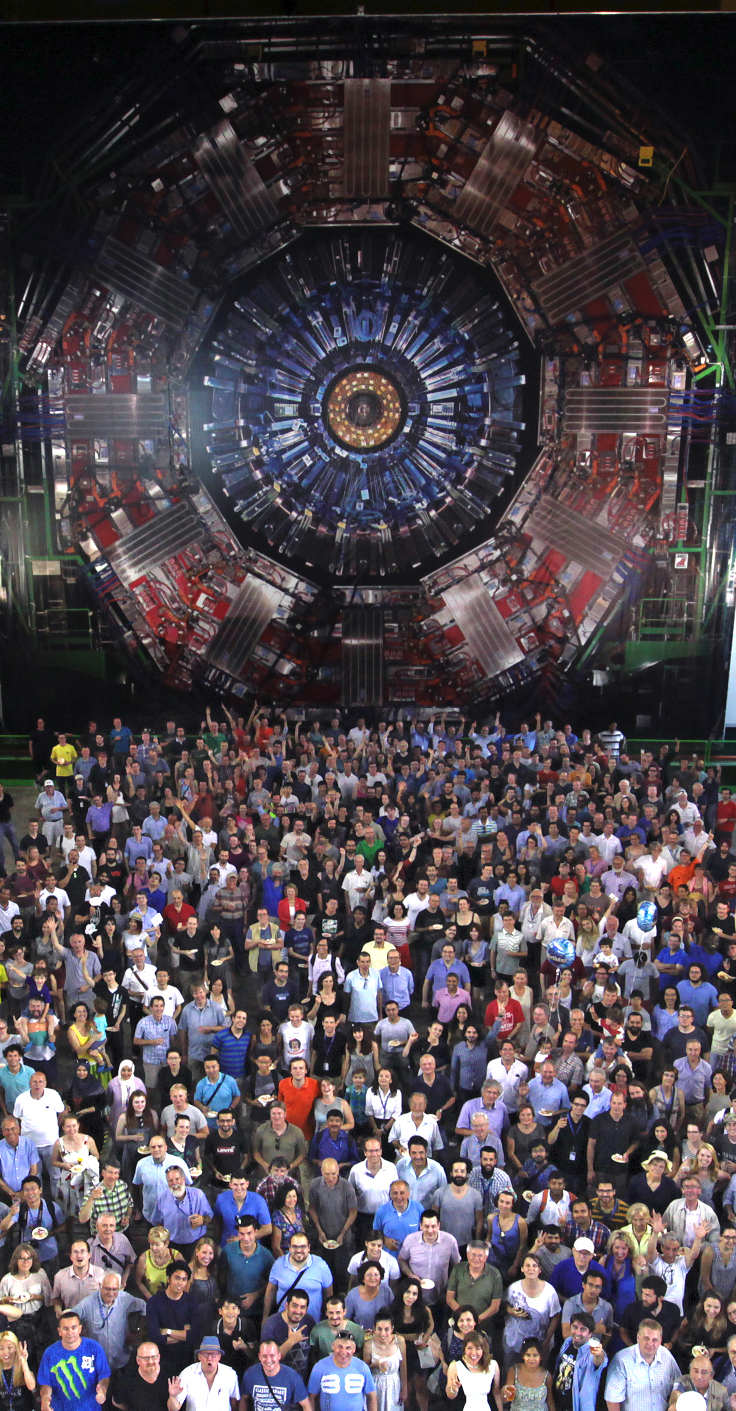
\includegraphics[width=\linewidth]{cms25_2.jpg}
\end{columns}
\end{frame}

\begin{frame}{Algorithm to identify a particle decay}
\large
\vspace{0.5 cm}
\begin{enumerate}
\item Loop over all pairs of particle tracks, tentatively labeling them $\pi^+$ and $\pi^-$.
\item Calculate m = $\sqrt{(E_{\pi^+} + E_{\pi^-})^2 - \left|\vec{p}_{\pi^+} + \vec{p}_{\pi^-}\right|^2}$ for each pair.
\item The ones with $m \sim \mbox{mass}({K_s^0}) = 0.5\mbox{ GeV}/c^2$ are good candidates.
\end{enumerate}

\begin{center}
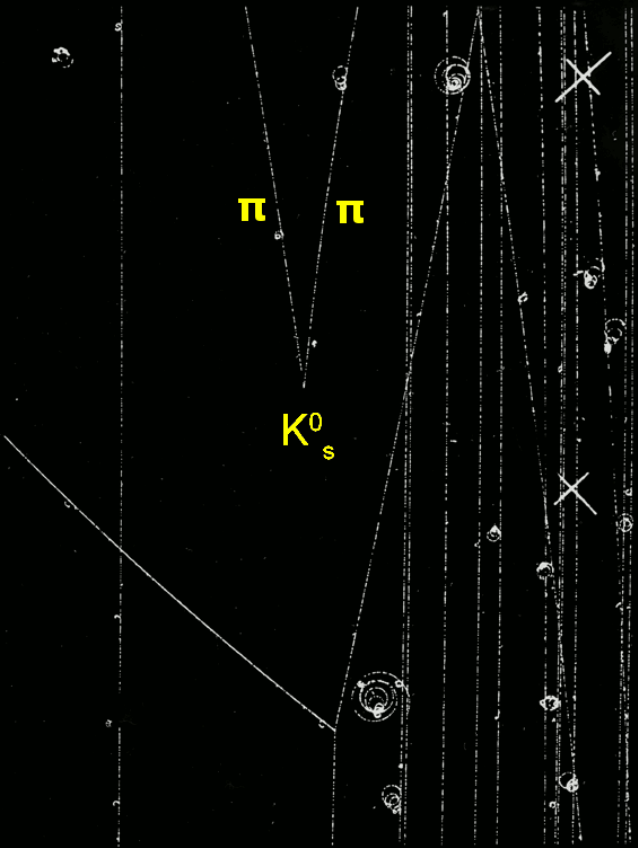
\includegraphics[height=4.2 cm]{kshort-1.png}\hspace{0.1 cm}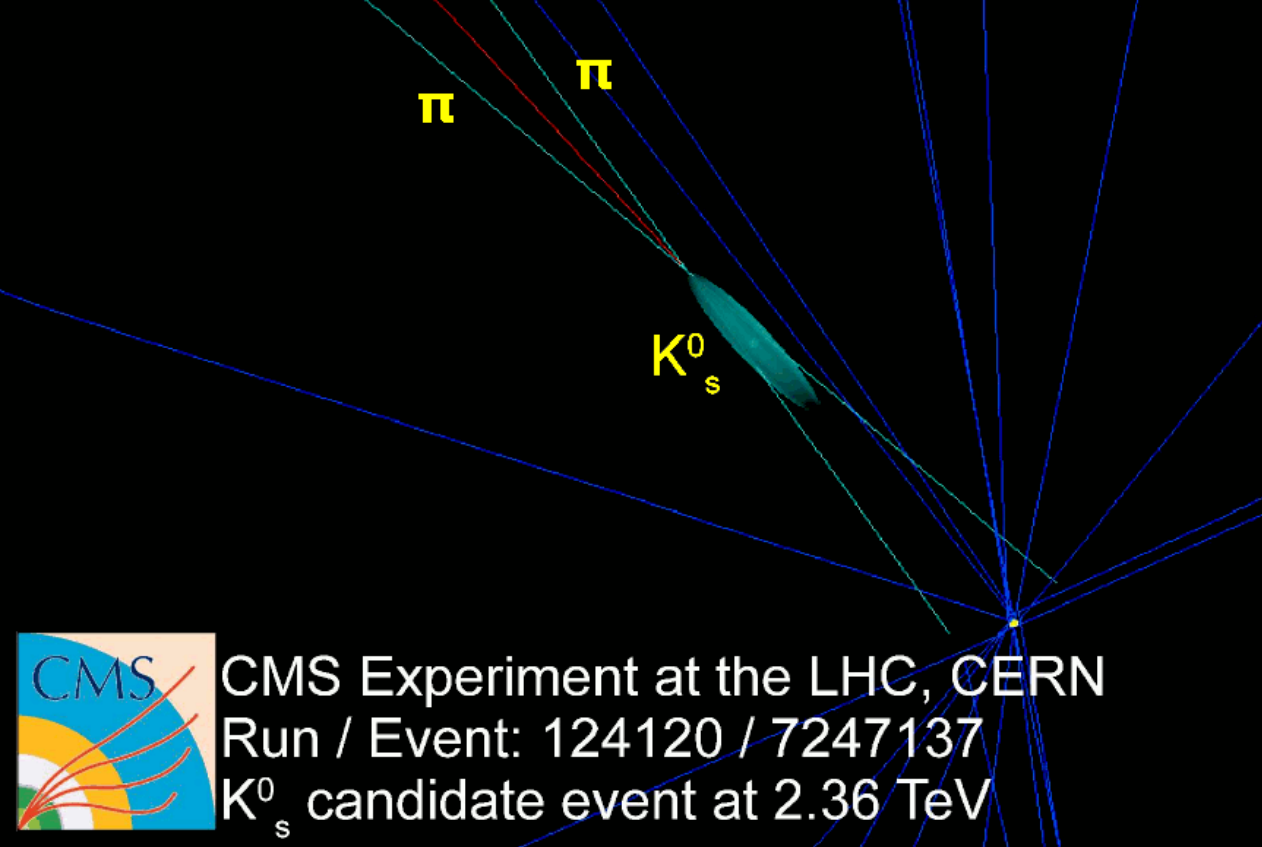
\includegraphics[height=4.2 cm]{kshort-2.png}\hspace{0.1 cm}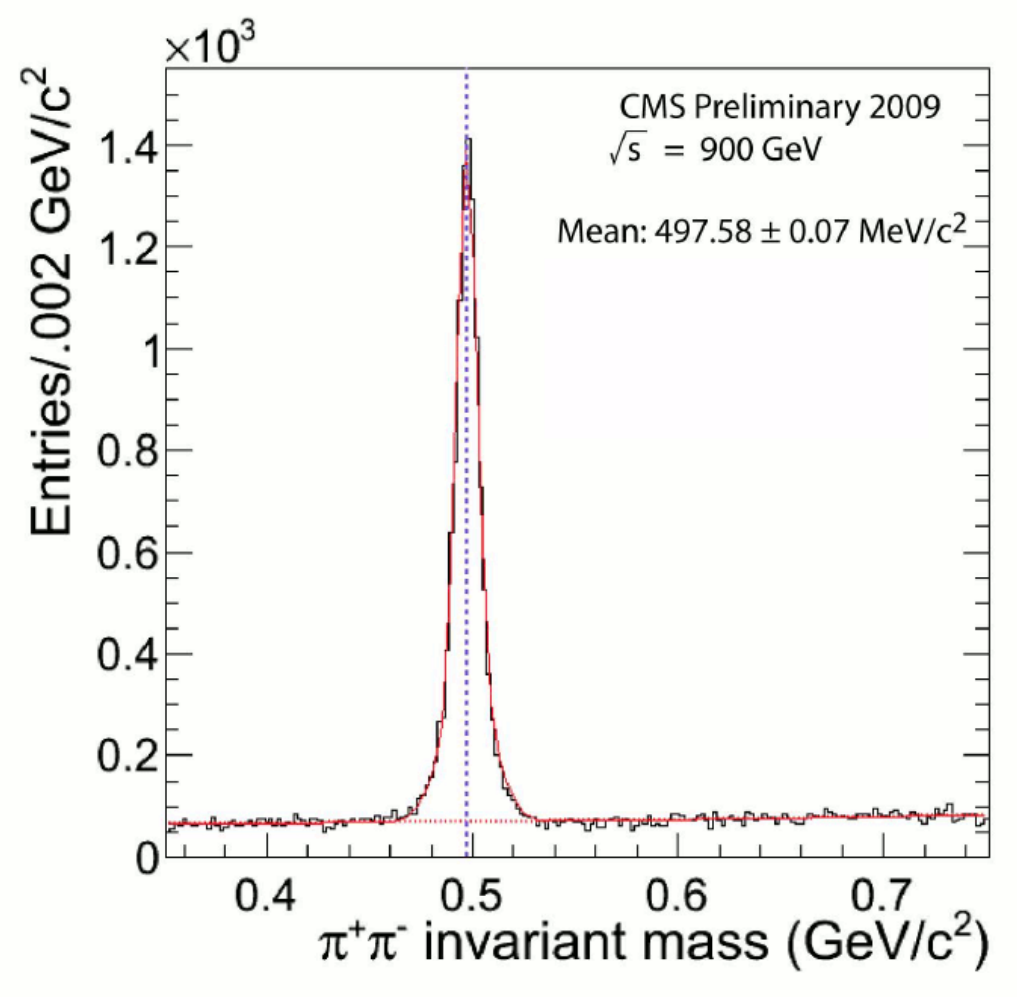
\includegraphics[height=4.2 cm]{kshort-3.png}
\end{center}
\end{frame}

\begin{frame}{Apply successively down the decay chain}
\Large
\begin{center}
$H \to ZZ$\hspace{1 cm}$Z \to e^+e^-$\hspace{1 cm}$Z \to \mu^+\mu^-$
\end{center}

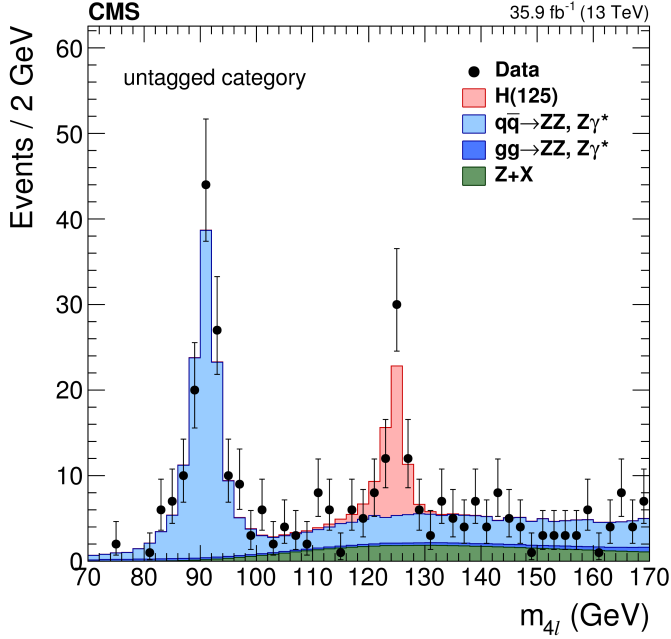
\includegraphics[height=6 cm]{higgs-to-four-leptons.png}\hfill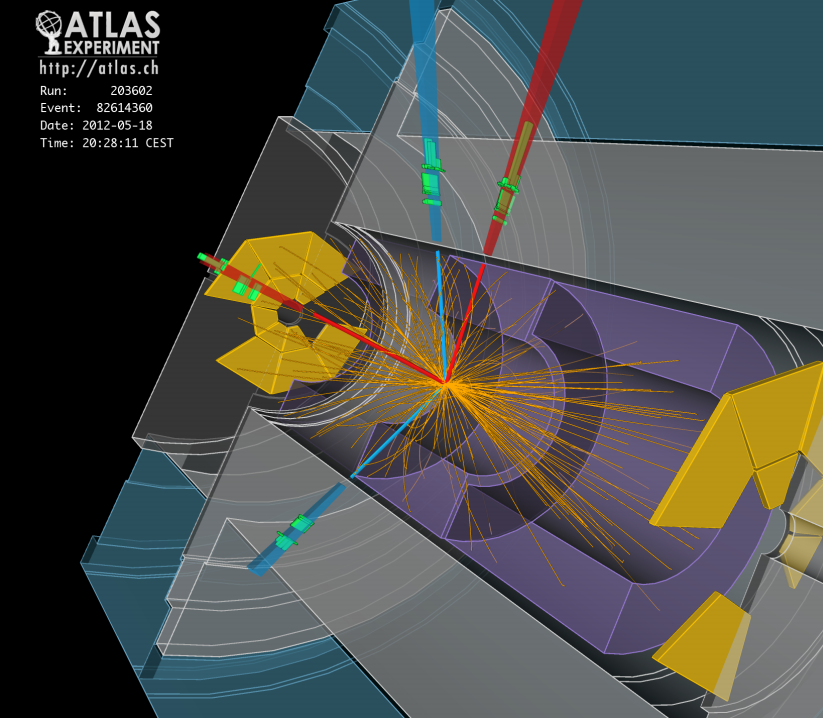
\includegraphics[height=6 cm]{higgs-to-four-leptons-2.png}
\end{frame}

\begin{frame}{Key parts of the calculation}
\Large
\vspace{0.15 cm}
\begin{itemize}\setlength{\itemsep}{0.25 cm}
\item All events are independent; no particles or decays cross from one event to the next.
\item Detectors produce collections of different kinds of signals: tracks, energy deposition, timing, etc., each in its own variable-length collection.
\item Candidates are generated with a \mintinline{sql}{SELF JOIN} (items from the same collection) or a \mintinline{sql}{CROSS JOIN} (items from different collections) \mintinline{sql}{ON t1.eventId == t2.eventId}.
\item Good candidates are identified by {\it filtering} (throw away the bad) and/or {\it reduction} (pick the best of what remains.)
\end{itemize}
\end{frame}

\begin{frame}{Key parts of the calculation}
\Large
\vspace{0.5 cm}
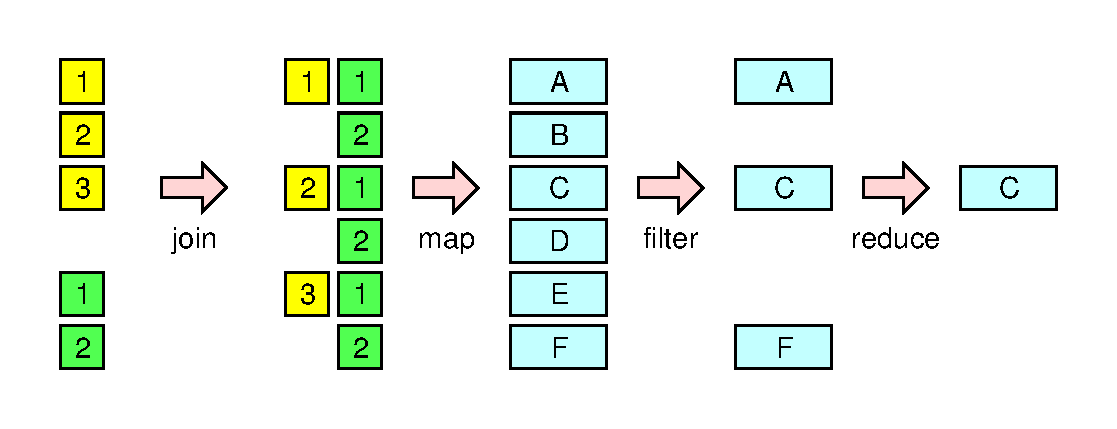
\includegraphics[width=\linewidth]{explode-flat-reduce.pdf}

\hfill \ldots independently for each event.
\end{frame}

\begin{frame}{Key part of the data structure}
\Large
\vspace{0.25 cm}
\begin{itemize}
\item Large number of events, processed in parallel.
\item Each event has an {\it arbitrary number} of record structures.
\item Not reducible to a flat table without padding and/or loss.
\end{itemize}

\vspace{0.25 cm}
\begin{columns}
\column{0.5\linewidth}
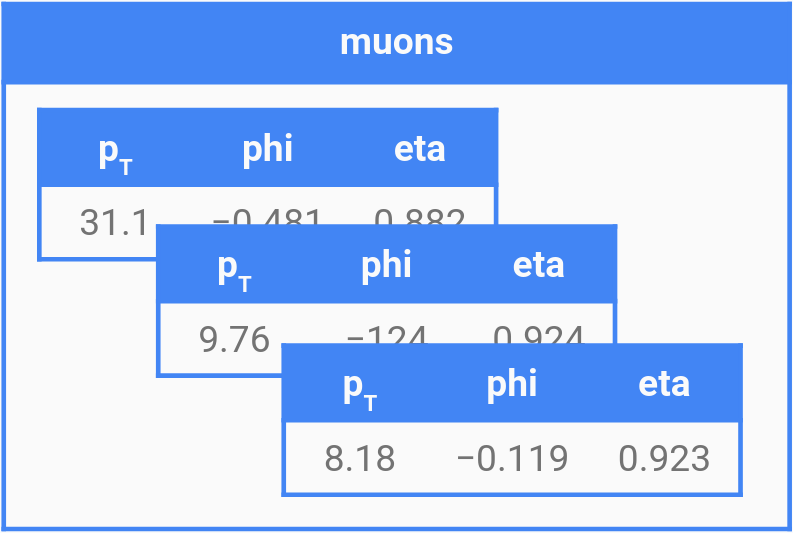
\includegraphics[width=\linewidth]{muons-as-objects.png}

\column{0.5\linewidth}
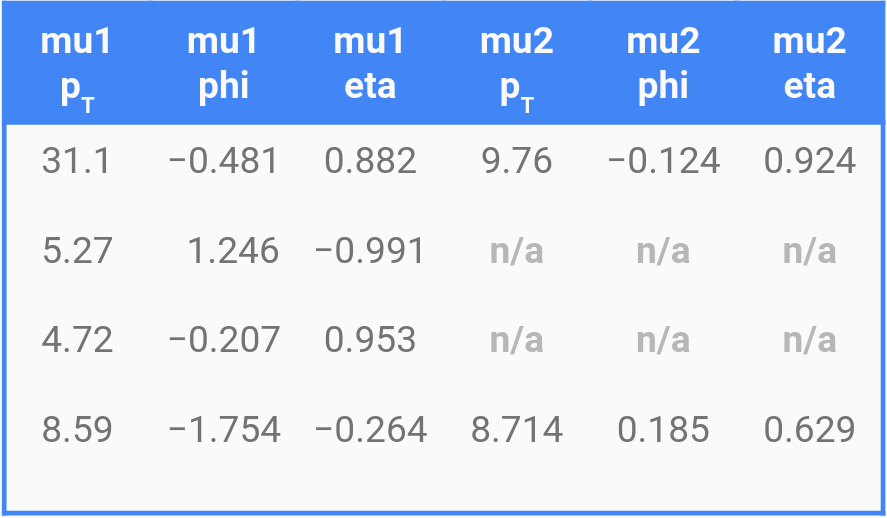
\includegraphics[width=\linewidth]{muons-as-a-table.png}
\end{columns}
\end{frame}

\begin{frame}{Programming languages used in particle physics}
\large
\vspace{0.5 cm}
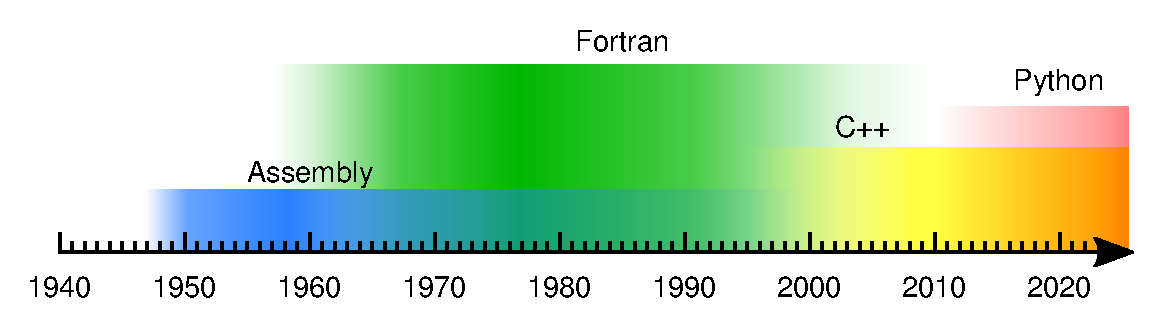
\includegraphics[width=\linewidth]{programming-languages.pdf}

\begin{itemize}\setlength{\itemsep}{0.2 cm}
\item First programmable computers were used for particle physics simulations.
\item Fortran was used to analyze events soon after the language was invented;

physicists wrote packages (BOS, HYDRA, ZBOOK) to add data structures.

\item Major transition from Fortran to C++ in the late 1990's/early 2000's.
\item Very recent adoption of Python (alongside C++).
\end{itemize}
\end{frame}

\begin{frame}{The Python transition is happening {\it right now}}
\vspace{0.2 cm}
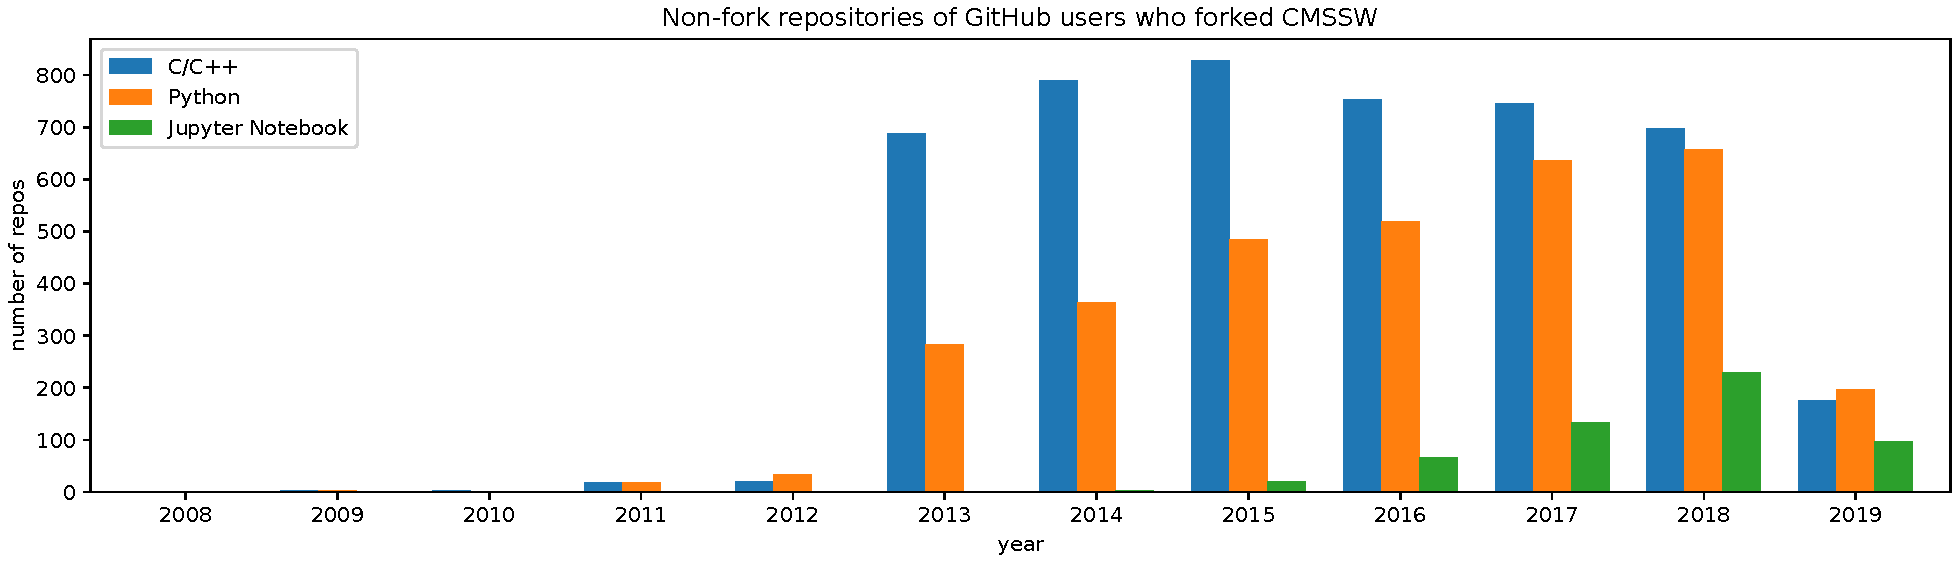
\includegraphics[width=\linewidth]{github-cmssw-lin.pdf}

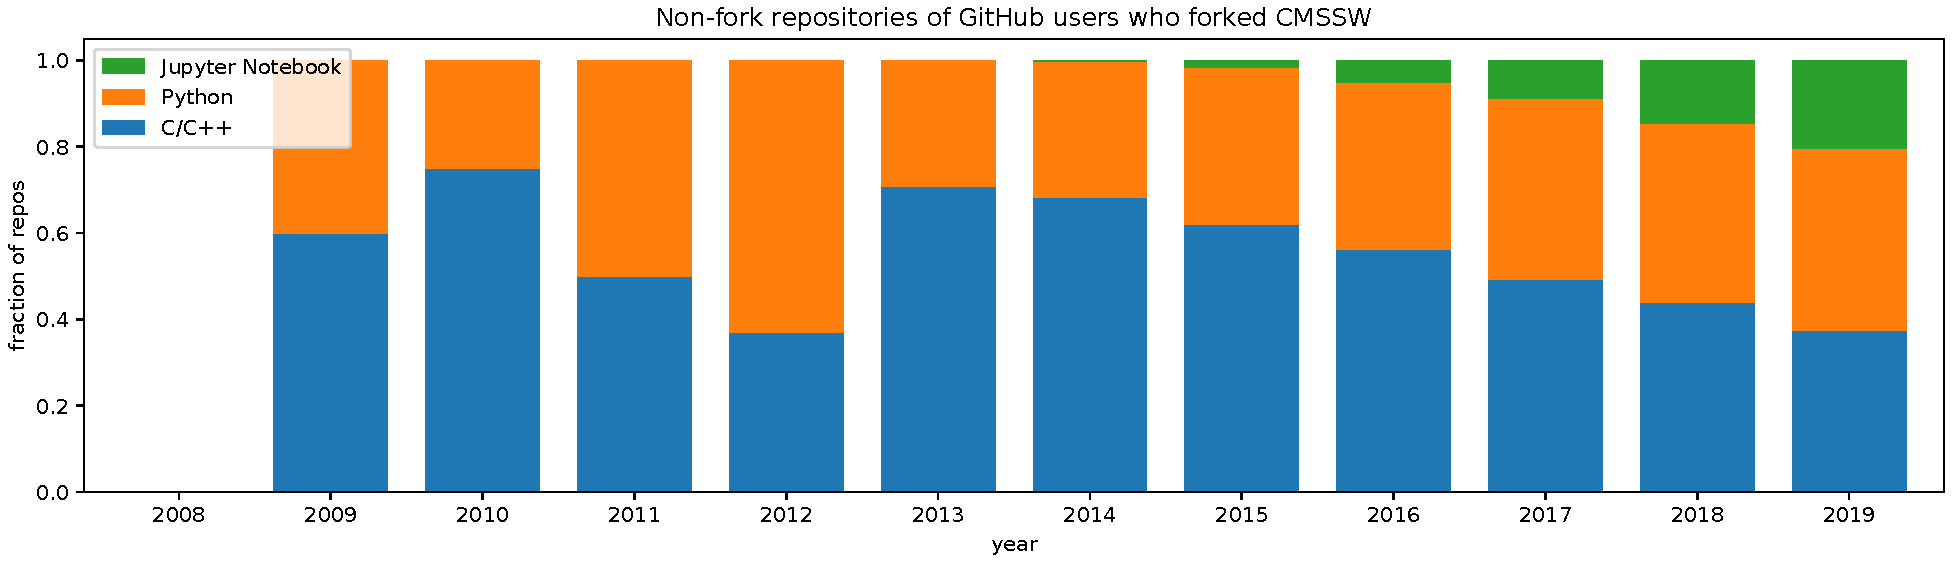
\includegraphics[width=\linewidth]{github-cmssw-frac.pdf}
\end{frame}

\begin{frame}[fragile]{In our field, ``conventional'' analysis means C++}
\vspace{0.25 cm}
\begin{columns}[b]
\column{0.7\linewidth}
\begin{minted}{c++}
std::vector<Kaon*> getKaons(Event event) {
  std::vector<Track*> tracks = event.getTracks();
  std::vector<Kaon*> kaons;
  for (auto t1 = tracks.begin(); t1 != tracks.end(); ++t1) {
    for (auto t2 = t1 + 1; t2 != tracks.end(); ++t2) {
      if (t1->charge != t2->charge) {
        double m = mass(t1, t2);
        if (fabs(m - 0.5) < 0.01) {
          kaons.push_back(new Kaon(t1, t2));
        }
      }
    }
  }
  return kaons;
}
\end{minted}

\vspace{0.1 cm}

\column{0.25\linewidth}
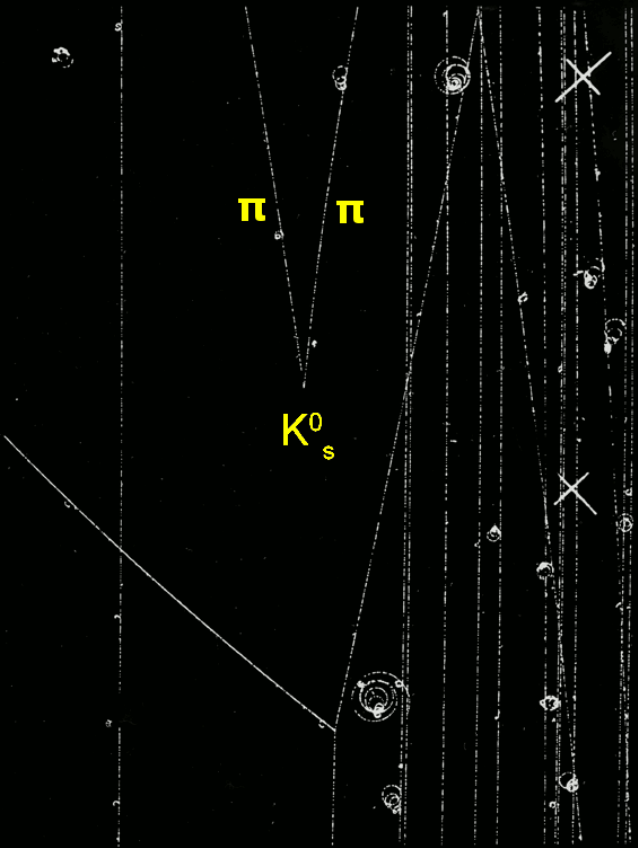
\includegraphics[width=\linewidth]{kshort-1.png}
\end{columns}
\end{frame}

\begin{frame}[fragile]{But direct translation to Python would be a performance disaster}
\vspace{0.25 cm}
\begin{columns}[b]
\column{0.7\linewidth}
\begin{minted}[stripnl=false]{python}
def getKaons(event):
  tracks = event.getTracks()
  kaons = []
  for i, t1 in enumerate(tracks):
    for t2 in tracks[i + 1:]:
      if t1.charge != t2.charge:
        m = mass(t1, t2)
        if abs(m - 0.5) < 0.01:
          kaons.append(Kaon(t1, t2))




  return kaons

\end{minted}

\vspace{0.1 cm}

\column{0.25\linewidth}
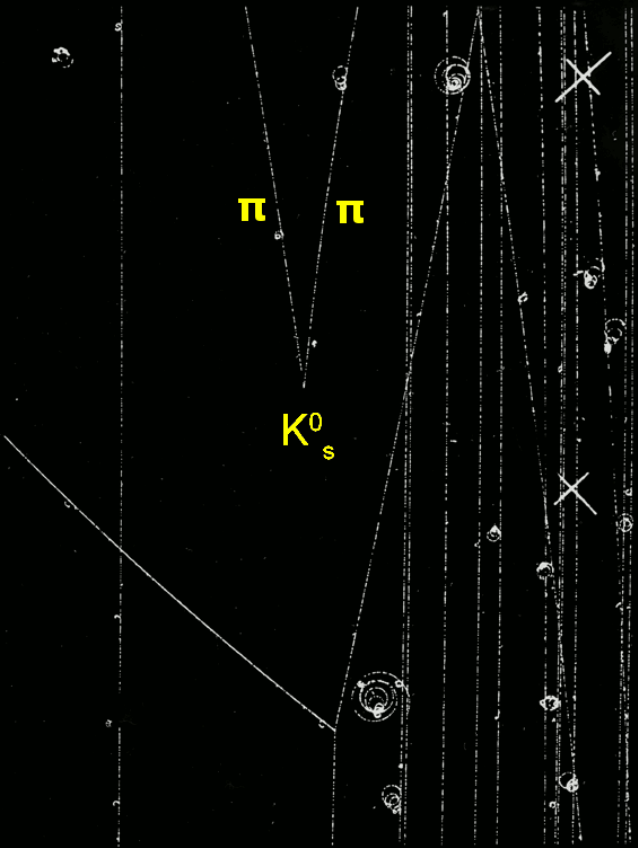
\includegraphics[width=\linewidth]{kshort-1.png}
\end{columns}
\end{frame}

\begin{frame}{High-performance processing in Python usually requires Numpy}
\vspace{0.5 cm}
\begin{center}

\includegraphics[width=0.35\linewidth]{numpy-logo.png}

\vspace{1 cm}
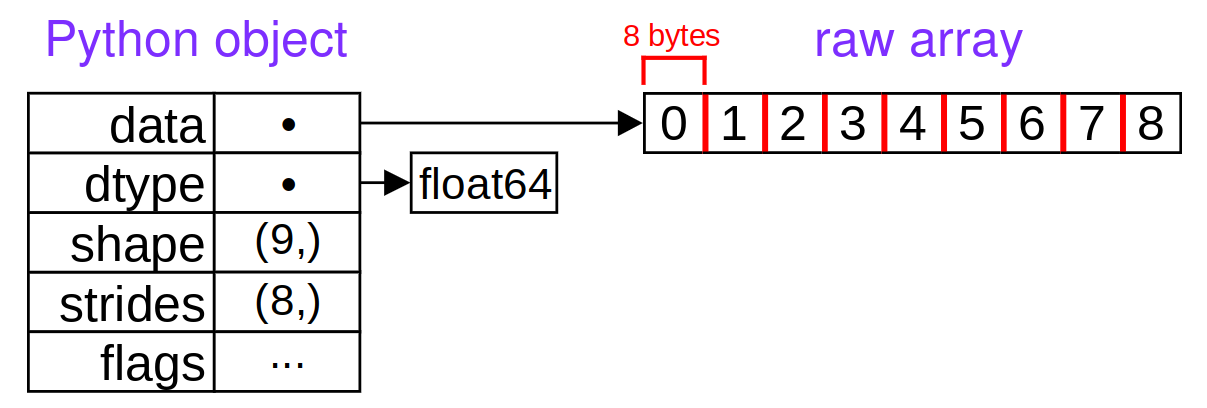
\includegraphics[width=0.75\linewidth]{numpy-memory-layout.png}
\end{center}
\end{frame}

\begin{frame}[fragile]{High-performance processing in Python usually requires Numpy}
\Large
\vspace{0.5 cm}
\begin{columns}
\column{0.52\linewidth}
Numpy has a suite of operations that each apply to whole arrays (compiled, maybe vectorized loop):

\small
\begin{minted}{python}
def calculate(pt, eta):
    pz = pt * numpy.sinh(eta)

calculate(pt_scalar, eta_scalar)
calculate(pt_array,  eta_array)
\end{minted}

\Large
\vspace{0.5 cm}

\uncover<2->{By manipulating the {\tt shape} and {\tt strides}, slices are $\mathcal{O}(1)$ and zero-copy.}

\column{0.4\linewidth}
\uncover<2->{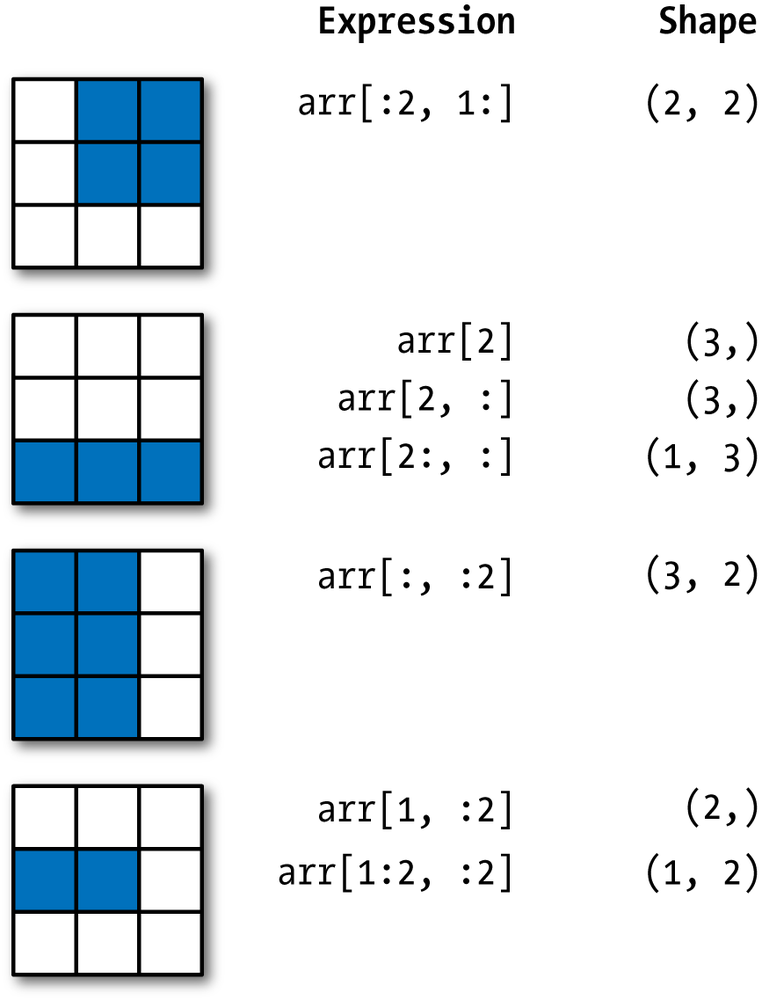
\includegraphics[width=\linewidth]{numpy-slicing.png}}
\end{columns}
\end{frame}

\begin{frame}{But Numpy doesn't have anything for variable-length lists}
\Large
\vspace{0.5 cm}
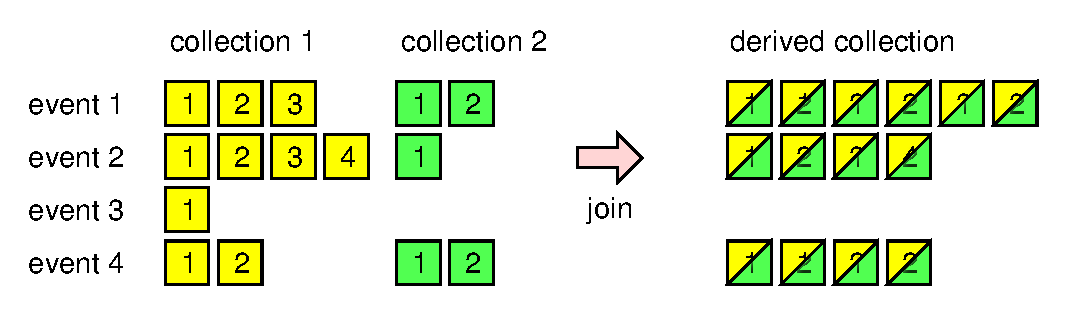
\includegraphics[width=\linewidth]{two-collections.pdf}

\vspace{0.5 cm}
\uncover<2->{Arrays of variable-length subarrays are sometimes called ``jagged`` or ``ragged`` arrays.}
\end{frame}

\begin{frame}[fragile]{Jagged/nested data can still be ``columnar''}
\vspace{0.5 cm}
\begin{columns}
\column{0.5\linewidth}
\small
\begin{Verbatim}[commandchars=\\\{\}]
[[Muon(\textcolor{darkgreen}{31.1}, \textcolor{darkorange}{-0.481}, \textcolor{blue}{0.882}),
      Muon(\textcolor{darkgreen}{9.76}, \textcolor{darkorange}{-0.124}, \textcolor{blue}{0.924}),
      Muon(\textcolor{darkgreen}{8.18}, \textcolor{darkorange}{-0.119}, \textcolor{blue}{0.923})],
 [Muon(\textcolor{darkgreen}{5.27}, \textcolor{darkorange}{1.246}, \textcolor{blue}{-0.991})],
 [Muon(\textcolor{darkgreen}{4.72}, \textcolor{darkorange}{-0.207}, \textcolor{blue}{0.953})],
 [Muon(\textcolor{darkgreen}{8.59}, \textcolor{darkorange}{-1.754}, \textcolor{blue}{-0.264}),
      Muon(\textcolor{darkgreen}{8.714}, \textcolor{darkorange}{0.185}, \textcolor{blue}{0.629})]
]
\end{Verbatim}
\column{0.35\linewidth}
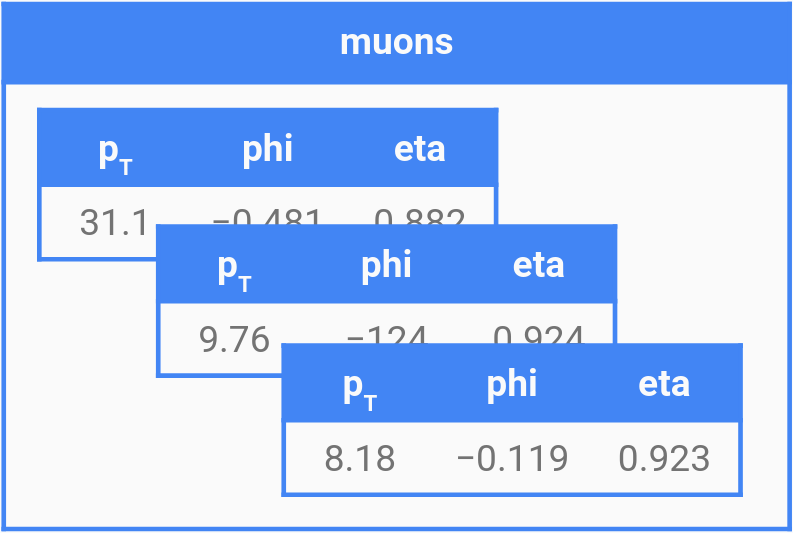
\includegraphics[width=\linewidth]{muons-as-objects.png}
\end{columns}
\vspace{0.5 cm}
They can be contiguous by field with \only<1>{\textcolor{red}{counts}}\only<2,3,4>{counts} or \only<2>{\textcolor{red}{offsets}}\only<1,3,4>{offsets} or \only<3>{\textcolor{red}{starts/stops}}\only<1,2,4>{starts/stops} or \only<4>{\textcolor{red}{parents}}\only<1,2,3>{parents} arrays.
\vspace{0.25 cm}
\begin{tabular}{r l}
\only<1>{\small \textcolor{red}{counts}  & \textcolor{red}{\tt\scriptsize \ \ \ \ \ 3,\ \ \ \ \ \ \ \ \ \ \ \ \ \ \ \ \ \ \ \ \ \ 1,\ \ \ \ \ \ 1,\ \ \ \ \ \ 2\ \ \ \ \ \ \ \ \ } \\}
\only<2>{\small \textcolor{red}{offsets} & \textcolor{red}{\tt\scriptsize \ \ \ \ \ 0,\ \ \ \ \ \ \ \ \ \ \ \ \ \ \ \ \ \ \ \ \ \ 3,\ \ \ \ \ \ 4,\ \ \ \ \ \ 5,\ \ \ \ \ \ \ 7} \\}
\only<4>{\small \textcolor{red}{parents} & \textcolor{red}{\tt\scriptsize \ \ \ \ \ 0,\ \ \ \ \ \ 0,\ \ \ \ \ \ 0,\ \ \ \ \ \ 1,\ \ \ \ \ \ 2,\ \ \ \ \ \ 3,\ \ \ \ \ 3} \\}
\only<3>{\small \textcolor{red}{starts}  & \textcolor{red}{\tt\scriptsize \ \ \ \ \ 0,\ \ \ \ \ \ \ \ \ \ \ \ \ \ \ \ \ \ \ \ \ \ 3,\ \ \ \ \ \ 4,\ \ \ \ \ \ 5\ \ \ \ \ \ \ \ \ } \\}
\uncover<3>{\small \textcolor{red}{stops}   & \textcolor{red}{\tt\scriptsize \ \ \ \ \ 3,\ \ \ \ \ \ \ \ \ \ \ \ \ \ \ \ \ \ \ \ \ \ 4,\ \ \ \ \ \ 5,\ \ \ \ \ \ 7\ \ \ \ \ \ \ \ \ } \\}
\small \mbox{\hspace{1 cm}$p_T$} & \textcolor{darkgreen}{\tt\scriptsize \ \ 31.1,\ \ \ 9.76,\ \ \ 8.18,\ \ \ 5.27,\ \ \ 4.72,\ \ \ 8.59, 8.714} \\
\small phi &  \textcolor{darkorange}{\tt\scriptsize -0.481,\ -0.123,\ -0.119,\ \ 1.246,\ -0.207,\ -1.754,\ 0.185} \\
\small eta &        \textcolor{blue}{\tt\scriptsize \ 0.882,\ \ 0.924,\ \ 0.923,\ -0.991,\ \ 0.953,\ -0.264,\ 0.629} \\
\end{tabular}
\end{frame}
\begin{frame}[fragile]{This provides efficient ways of {\it manipulating} data}
\vspace{0.25 cm}
``Remove the first muon from each event.'' \uncover<2->{\textcolor{red}{$\longrightarrow$ rewrite all inner lists.}}
\scriptsize
\begin{onlyenv}<1>
\begin{Verbatim}[commandchars=\\\{\}]
[[Muon(\textcolor{darkgreen}{31.1}, \textcolor{darkorange}{-0.481}, \textcolor{blue}{0.882}), Muon(\textcolor{darkgreen}{9.76}, \textcolor{darkorange}{-0.124}, \textcolor{blue}{0.924}), Muon(\textcolor{darkgreen}{8.18}, \textcolor{darkorange}{-0.119}, \textcolor{blue}{0.923})],
 [Muon(\textcolor{darkgreen}{5.27}, \textcolor{darkorange}{1.246}, \textcolor{blue}{-0.991})],
 [Muon(\textcolor{darkgreen}{4.72}, \textcolor{darkorange}{-0.207}, \textcolor{blue}{0.953})],
 [Muon(\textcolor{darkgreen}{8.59}, \textcolor{darkorange}{-1.754}, \textcolor{blue}{-0.264}), Muon(\textcolor{darkgreen}{8.714}, \textcolor{darkorange}{0.185}, \textcolor{blue}{0.629})],
 ...
\end{Verbatim}
\end{onlyenv}\begin{onlyenv}<2->
\begin{Verbatim}[commandchars=\\\{\}]
[[     \textcolor{darkgreen}{    }  \textcolor{darkorange}{      }  \textcolor{blue}{     }   Muon(\textcolor{darkgreen}{9.76}, \textcolor{darkorange}{-0.124}, \textcolor{blue}{0.924}), Muon(\textcolor{darkgreen}{8.18}, \textcolor{darkorange}{-0.119}, \textcolor{blue}{0.923})],
 [     \textcolor{darkgreen}{    }  \textcolor{darkorange}{     }  \textcolor{blue}{      } ],
 [     \textcolor{darkgreen}{    }  \textcolor{darkorange}{      }  \textcolor{blue}{     } ],
 [     \textcolor{darkgreen}{    }  \textcolor{darkorange}{      }  \textcolor{blue}{      }   Muon(\textcolor{darkgreen}{8.714}, \textcolor{darkorange}{0.185}, \textcolor{blue}{0.629})],
 ...
\end{Verbatim}
\end{onlyenv}
\normalsize
\vspace{0.5 cm}
``Remove the first muon from each event.'' \uncover<2->{\textcolor{red}{$\longrightarrow$ increase all starts by 1.}}
\vspace{0.25 cm}
\begin{onlyenv}<1>
\begin{tabular}{r l}
\small starts  &                    {\tt\scriptsize \ \ \ \ \ 0,\ \ \ \ \ \ \ \ \ \ \ \ \ \ \ \ \ \ \ \ \ \ 3,\ \ \ \ \ \ 4,\ \ \ \ \ \ 5\ \ \ \ \ \ \ \ \ } \\
\small stops   &                    {\tt\scriptsize \ \ \ \ \ 3,\ \ \ \ \ \ \ \ \ \ \ \ \ \ \ \ \ \ \ \ \ \ 4,\ \ \ \ \ \ 5,\ \ \ \ \ \ 7\ \ \ \ \ \ \ \ \ } \\
\small $p_T$ & \textcolor{darkgreen}{\tt\scriptsize \ \ 31.1,\ \ \ 9.76,\ \ \ 8.18,\ \ \ 5.27,\ \ \ 4.72,\ \ \ 8.59, 8.714} \\
\small phi &  \textcolor{darkorange}{\tt\scriptsize -0.481,\ -0.123,\ -0.119,\ \ 1.246,\ -0.207,\ -1.754,\ 0.185} \\
\small eta &        \textcolor{blue}{\tt\scriptsize \ 0.882,\ \ 0.924,\ \ 0.923,\ -0.991,\ \ 0.953,\ -0.264,\ 0.629} \\
\end{tabular}
\end{onlyenv}\begin{onlyenv}<2->
\begin{tabular}{r l}
\small starts  &     \textcolor{red}{\tt\scriptsize \ \ \ \ \ 1,\ \ \ \ \ \ \ \ \ \ \ \ \ \ \ \ \ \ \ \ \ \ 4,\ \ \ \ \ \ 5,\ \ \ \ \ \ 6\ \ \ \ \ \ \ \ \ } \\
\small stops   &                    {\tt\scriptsize \ \ \ \ \ 3,\ \ \ \ \ \ \ \ \ \ \ \ \ \ \ \ \ \ \ \ \ \ 4,\ \ \ \ \ \ 5,\ \ \ \ \ \ 7\ \ \ \ \ \ \ \ \ } \\
\small $p_T$ & \textcolor{darkgreen}{\tt\scriptsize \ \ 31.1,\ \ \ 9.76,\ \ \ 8.18,\ \ \ 5.27,\ \ \ 4.72,\ \ \ 8.59, 8.714} \\
\small phi &  \textcolor{darkorange}{\tt\scriptsize -0.481,\ -0.123,\ -0.119,\ \ 1.246,\ -0.207,\ -1.754,\ 0.185} \\
\small eta &        \textcolor{blue}{\tt\scriptsize \ 0.882,\ \ 0.924,\ \ 0.923,\ -0.991,\ \ 0.953,\ -0.264,\ 0.629} \\
\end{tabular}\end{onlyenv}
\vspace{0.5 cm}

\uncover<3>{We didn't need to touch any contents (i.e.\ read them from disk, decompress them\ldots).}
\end{frame}

\begin{frame}{Properties of this representation}
\Large
\vspace{0.5 cm}
\begin{itemize}\setlength{\itemsep}{0.5 cm}
\item<1-> Data structures are {\it fully composable:} a jagged array's content can be another jagged array, some fields of a record structure can be jagged, others not.
\item<2-> Most operations (such as slicing) can modify the structure ({\tt counts}/{\tt offsets}/{\tt starts,stops}/{\tt parents}) without touching the content.
\end{itemize}
\end{frame}

%% \begin{frame}{Example: generate distinct muon pairs}
%% \vspace{0.2 cm}

%% \begin{columns}
%% \column{1.1\linewidth}

%% {\large\bf muons:}

%% \vspace{0.2 cm}
%% \begin{tabular}{r l}
%% \textcolor{red}{counts}  & \textcolor{red}{\tt \ \ \ \ \ 3,\ \ \ \ \ \ \ \ \ \ \ \ \ \ \ \ \ \ \ \ \ \ 1,\ \ \ \ \ \ 1,\ \ \ \ \ \ 2\ \ \ \ \ \ \ \ \ } \\
%% \textcolor{red}{offsets} & \textcolor{red}{\tt \ \ \ \ \ 0,\ \ \ \ \ \ \ \ \ \ \ \ \ \ \ \ \ \ \ \ \ \ 3,\ \ \ \ \ \ 4,\ \ \ \ \ \ 5,\ \ \ \ \ \ \ 7} \\
%% \textcolor{red}{starts}  & \textcolor{red}{\tt \ \ \ \ \ 0,\ \ \ \ \ \ \ \ \ \ \ \ \ \ \ \ \ \ \ \ \ \ 3,\ \ \ \ \ \ 4,\ \ \ \ \ \ 5\ \ \ \ \ \ \ \ \ } \\
%% \textcolor{red}{stops}   & \textcolor{red}{\tt \ \ \ \ \ 3,\ \ \ \ \ \ \ \ \ \ \ \ \ \ \ \ \ \ \ \ \ \ 4,\ \ \ \ \ \ 5,\ \ \ \ \ \ 7\ \ \ \ \ \ \ \ \ } \\
%% \mbox{\hspace{1 cm}$p_T$} & \textcolor{darkgreen}{\tt \ \ 31.1,\ \ \ 9.76,\ \ \ 8.18,\ \ \ 5.27,\ \ \ 4.72,\ \ \ 8.59, 8.714} \\
%% phi &  \textcolor{darkorange}{\tt -0.481,\ -0.123,\ -0.119,\ \ 1.246,\ -0.207,\ -1.754,\ 0.185} \\
%% eta &        \textcolor{blue}{\tt \ 0.882,\ \ 0.924,\ \ 0.923,\ -0.991,\ \ 0.953,\ -0.264,\ 0.629} \\
%% \end{tabular}

%% \vspace{0.6 cm}
%% {\large\bf muons.choose(2):}

%% \vspace{0.2 cm}
%% \begin{tabular}{r l}
%% \textcolor{red}{counts}  &   \textcolor{red}{\tt 3,\ \ \ \ \ \ \ 0,\ 0,\ 1} \\
%% \textcolor{red}{offsets} &   \textcolor{red}{\tt 0,\ \ \ \ \ \ \ 2,\ 2,\ 2,\ 3} \\
%% \textcolor{black}{left}  & \textcolor{black}{\tt 0,\ 0,\ 1,\ \ \ \ \ \ \ 5} \\
%% \textcolor{black}{right} & \textcolor{black}{\tt 1,\ 2,\ 2,\ \ \ \ \ \ \ 6} \\
%% \textcolor{black}{left.content}  & \textcolor{black}{muons} \\
%% \textcolor{black}{right.content} & \textcolor{black}{muons} \\
%% \end{tabular}

%% \vspace{-3.2 cm}
%% \uncover<2->{\hfill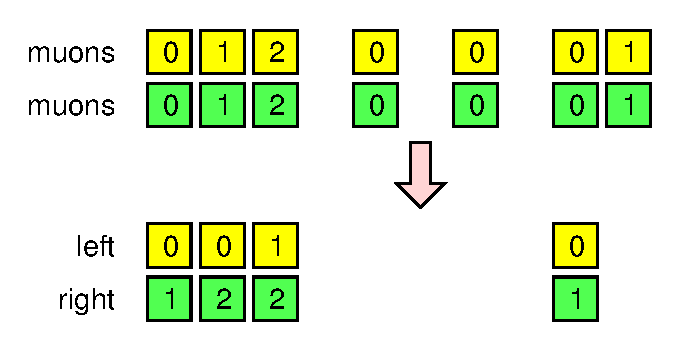
\includegraphics[height=3.5 cm]{muons-choose-2.pdf}}

%% \vspace{0.2 cm}
%% \uncover<3->{\textcolor{gray}{(The ``left'' and ``right'' of each pair is a link to the original muons.)}}
%% \end{columns}
%% \end{frame}

%% \begin{frame}[fragile]{As a data structure}
%% \vspace{0.25 cm}
%% \begin{columns}
%% \column{1.08\linewidth}
%% \scriptsize
%% \begin{verbatim}
%% muons =
%%     ListArray(
%%         offsets = [0, 3, 4, 5, 7],
%%         content =
%%             RecordArray(
%%                  pT = numpy.array([  31.1,   9.76,   8.18,   5.27,   4.72,   8.59, 8.714]),
%%                 eta = numpy.array([-0.481, -0.123, -0.119,  1.246, -0.207, -1.754, 0.185]),
%%                 phi = numpy.array([ 0.882,  0.924,  0.923, -0.991,  0.953, -0.264, 0.629])))



%% muons.choose(2) =
%%     ListArray(
%%         offsets = [0, 2, 2, 2, 3],
%%         content =
%%             RecordArray(
%%                  left = IndirectArray(index = [0, 0, 1, 5], content = muons)
%%                 right = IndirectArray(index = [1, 2, 2, 6], content = muons)))
%% \end{verbatim}
%% \end{columns}
%% \end{frame}

\begin{frame}[fragile]{Awkward Array: data structures with a Numpy-like interface}
\small
\hfill
\includegraphics[height=2 cm]{awkward-logo.pdf}

\vspace{-2 cm}
\begin{minted}{python}
>>> import awkward
>>> array = awkward.fromiter(
...     [[1.1, 2.2, None, 3.3, None],
...      [4.4, [5.5]],
...      [{"x": 6, "y": {"z": 7}}, None, {"x": 8, "y": {"z": 9}}]])
\end{minted}

\begin{uncoverenv}<2->
\begin{minted}{python}
>>> print(array)
[[1.1 2.2 None 3.3 None] [4.4 [5.5]] [<Row 0> None <Row 1>]]
\end{minted}
\end{uncoverenv}

\begin{uncoverenv}<3->
\begin{minted}{python}
>>> print(array[:, -2:])    # get whole outer list, last two of inner
[[3.3 None] [4.4 [5.5]] [None <Row 1>]]
\end{minted}
\end{uncoverenv}

\begin{uncoverenv}<4->
\begin{minted}{python}
>>> (array + 100).tolist()  # element-wise function applied to arrays
[[101.1, 102.2, None, 103.3, None],
 [104.4, [105.5]],
 [{'x': 106, 'y': {'z': 107}}, None, {'x': 108, 'y': {'z': 109}}]]
\end{minted}
\end{uncoverenv}
\end{frame}

\begin{frame}[fragile]{Internally, it's a bunch or Numpy arrays {\it interpreted} as nested data}
\begin{columns}
\column{1.1\linewidth}
\scriptsize
\begin{minted}{python}
>>> array.layout
 layout
[           ()] JaggedArray(starts=layout[0], stops=layout[1], content=layout[2])
[            0]   ndarray(shape=3, dtype=dtype('int64'))
[            1]   ndarray(shape=3, dtype=dtype('int64'))
[            2]   IndexedMaskedArray(mask=layout[2, 0], content=layout[2, 1], maskedwhen=-1)
[         2, 0]     ndarray(shape=10, dtype=dtype('int64'))
[         2, 1]     UnionArray(tags=layout[2, 1, 0], index=layout[2, 1, 1],
                               contents=[layout[2, 1, 2], layout[2, 1, 3], layout[2, 1, 4]])
[      2, 1, 0]       ndarray(shape=7, dtype=dtype('uint8'))
[      2, 1, 1]       ndarray(shape=7, dtype=dtype('int64'))
[      2, 1, 2]       ndarray(shape=4, dtype=dtype('float64'))
[      2, 1, 3]       JaggedArray(starts=layout[2, 1, 3, 0], stops=layout[2, 1, 3, 1],
                                  content=layout[2, 1, 3, 2])
[   2, 1, 3, 0]         ndarray(shape=1, dtype=dtype('int64'))
[   2, 1, 3, 1]         ndarray(shape=1, dtype=dtype('int64'))
[   2, 1, 3, 2]         ndarray(shape=1, dtype=dtype('float64'))
[      2, 1, 4]       Table(x=layout[2, 1, 4, 0], y=layout[2, 1, 4, 1])
[   2, 1, 4, 0]         ndarray(shape=2, dtype=dtype('int64'))
[   2, 1, 4, 1]         Table(z=layout[2, 1, 4, 1, 0])
[2, 1, 4, 1, 0]           ndarray(shape=2, dtype=dtype('int64'))
\end{minted}
\end{columns}
\end{frame}

\begin{frame}[fragile]{High-level type may be described by what \mintinline{python}{array[x]} returns}
\small
\begin{minted}{python}
>>> print(array.type)
[0, 3) -> [0, inf) -> ?((float64             |
                         [0, inf) -> float64 |
                         'x' -> int64
                         'y' -> 'z' -> int64 ))
\end{minted}

\normalsize
\vspace{0.5 cm}
{\bf That is,}
\begin{itemize}
\item first square bracket in \mintinline{python}{array[x]} takes a non-negative integer less than 3;
\item second takes a non-negative integer (unknown upper limit because it's jagged);
\item what that returns is nullable (might be \mintinline{python}{None});
\item and it could be a \mintinline{python}{float}, a jagged array of floats, or a record taking \mintinline{python}{'x'} or \mintinline{python}{'y'};
\item \mintinline{python}{'x'} returns an integer; \mintinline{python}{'y'} returns another record taking \mintinline{python}{'z'} to integers.
\end{itemize}
\end{frame}

\begin{frame}[fragile]{NASA exoplanets dataset: stars may have more than one planet}
\begin{columns}
\column{1.09\linewidth}
\small
\begin{minted}{python}
>>> import urllib.request
>>> stars = awkward.fromiter(
...     json.load(
...         urllib.request.urlopen(
...            "http://scikit-hep.org/uproot/examples/exoplanets.json")))
\end{minted}

\begin{onlyenv}<1>
\begin{minted}{python}
>>> stars
<Table [<Row 0> <Row 1> <Row 2> ... <Row 2933> <Row 2934>]>
\end{minted}

\vspace{10 cm}
\end{onlyenv}
\begin{onlyenv}<2>
\begin{minted}{python}
>>> stars[8:10].tolist()
[{'name': '24 Sex', 'ra': 155.86821, 'dec': -0.902244, 'dist': 72.21,
  'mass': 1.54, 'radius': 4.9, 'planets': [
      {'name': 'b', 'orbit': 1.333, 'eccen': 0.09, 'period': 452.8,
       'mass': 1.99, 'radius': None},
      {'name': 'c', 'orbit': 2.08, 'eccen': 0.29, 'period': 883.0,
       'mass': 0.86, 'radius': None}]},
 {'name': '2MASS J01225093-2439505', 'ra': 20.712243, 'dec': -24.664049,
  'dist': 36.0, 'mass': 0.4, 'radius': None, 'planets': [
      {'name': 'b', 'orbit': 52.0, 'eccen': None, 'period': None,
       'mass': 24.5, 'radius': None}]}
]
\end{minted}

\vspace{10 cm}
\end{onlyenv}
\begin{onlyenv}<3>
\small
\vspace{-0.5 cm}
\begin{verbatim}
>>> print(stars.type)
[0, 2935) -> 'name'    -> <class 'str'>
             'ra'      -> float64
             'dec'     -> float64
             'dist'    -> ?(float64)
             'mass'    -> ?(float64)
             'radius'  -> ?(float64)
             'planets' -> [0, inf) -> 'name'   -> <class 'str'>
                                      'orbit'  -> ?(float64)
                                      'eccen'  -> ?(float64)
                                      'period' -> ?(float64)
                                      'mass'   -> ?(float64)
                                      'radius' -> ?(float64)
\end{verbatim}

\vspace{10 cm}
\end{onlyenv}
\begin{onlyenv}<4-5>
\begin{minted}{python}
>>> stars["mass"]
<MaskedArray [2.7 2.78 2.2 ... 2.3 1.3 2.2]>

>>> stars["planets"]["mass"]
<JaggedArray [[19.4] [14.74] [4.8] ... [20.6] [0.6876 1.981 4.132] [2.8]]>
\end{minted}

\begin{uncoverenv}<5>
\begin{minted}{python}
>>> print(stars["mass"].type)             # just selecting a column
[0, 2935) -> ?(float64)
>>> print(stars["planets"]["mass"].type)  # projecting through a column
[0, 2935) -> [0, inf) -> ?(float64)
\end{minted}
\end{uncoverenv}

\vspace{10 cm}
\end{onlyenv}
\begin{onlyenv}<6>
\begin{minted}{python}
>>> stars[8]["planets"][1]["mass"]        # int and str indexes commute!
0.86
>>> stars[8]["planets"]["mass"][1]
0.86
>>> stars["planets"][8][1]["mass"]
0.86
>>> stars["planets"][8]["mass"][1]
0.86
>>> stars["planets"]["mass"][8][1]
0.86
\end{minted}

\vspace{10 cm}
\end{onlyenv}
\begin{onlyenv}<7>
\vspace{-0.4 cm}
\begin{minted}{python}
>>> awkward.topandas(stars, flatten=True)
\end{minted}

\tiny
\vspace{-0.6 cm}
\begin{verbatim}
            name          ra        dec    dist  mass radius planets                                               
                                                                name     orbit   eccen       period    mass radius
0    0    11 Com  185.179276  17.792868   93.37  2.70  19.00       b  1.290000  0.2310   326.03000  19.4000    NaN
1    0    11 UMi  229.274536  71.823898  125.72  2.78  29.79       b  1.530000  0.0800   516.21997  14.7400    NaN
2    0    14 And  352.822571  39.236198   75.59  2.20  11.00       b  0.830000  0.0000   185.84000   4.8000    NaN
3    0    14 Her  242.601303  43.817646   17.94  0.90   0.93       b  2.930000  0.3700  1773.40002   4.6600    NaN
4    0  16 Cyg B  295.466553  50.517525   21.41  1.08   1.13       b  1.660000  0.6800   798.50000   1.7800    NaN
5    0    18 Del  314.608063  10.839286   76.38  2.30   8.50       b    2.600   0.080    993.30000  10.3000    NaN
6    0  1RXS J16  242.376268 -21.083036  145.00  0.85   0.00       b  330.000     NaN          NaN   8.0000    NaN
7    0    24 Boo  217.157547  49.844852   96.25  0.99  10.64       b    0.190   0.042     30.35060   0.9100    NaN
8    0    24 Sex  155.868210  -0.902244   72.21  1.54   4.90       b    1.333   0.090    452.80000   1.9900    NaN
     1    24 Sex  155.868210  -0.902244   72.21  1.54   4.90       c    2.080   0.290    883.00000   0.8600    NaN
...          ...         ...        ...     ...   ...    ...     ...       ...     ...         ...      ...    ...
2932 0   tau Gem  107.784882  30.245163  112.64  2.30  26.80       b  1.170000  0.0310   305.500000 20.6000    NaN
2933 0   ups And   24.199345  41.405460   13.41  1.30   1.56       b  0.059222  0.0215     4.617033  0.6876    NaN
     1   ups And   24.199345  41.405460   13.41  1.30   1.56       c  0.827774  0.2596   241.258000  1.9810    NaN
     2   ups And   24.199345  41.405460   13.41  1.30   1.56       d  2.513290  0.2987  1276.460000  4.1320    NaN
2934 0    xi Aql  298.562012   8.461452   56.27  2.20  12.00       b  0.680000  0.0000   136.750000  2.8000    NaN

[3933 rows x 12 columns]
\end{verbatim}

\vspace{10 cm}
\end{onlyenv}
\end{columns}
\end{frame}










\begin{frame}{}
\end{frame}

\end{document}
